% Following figures are from /Users/zang/Desktop/fit_results/fit_taunub_sys_1l_allVR_BONLY_MU3000_gU2_5_23L1_0_noWeights_N_minus_1_fullRegion_v3_HEPData/Plots/
% Source files: topVR_1tau0l2b_Res*_postFit.eps and topVR_1tau0l2b_Res*_postfit.yaml.
% Local verified copies: data/ch8/hepdata_20260924/ (Plots, Histograms, Fits).
% Styling: scripts/ch8/restyle_hepdata.py --family vr; native data and ratio drawings are preserved.
% Verification: output/ch8/hepdata_vr_update_20260924/figures.json.
% Axis notation/font update: scripts/ch8/axis_labels.py; output/ch8/axis_labels_20260924/.
% Previous version: figures_vrtop_bonly_20260921.tex (selected by \CHEightCRFigureVersion).
\begin{figure}[htpb]
    \centering
    \begin{subfigure}{0.49\linewidth}
        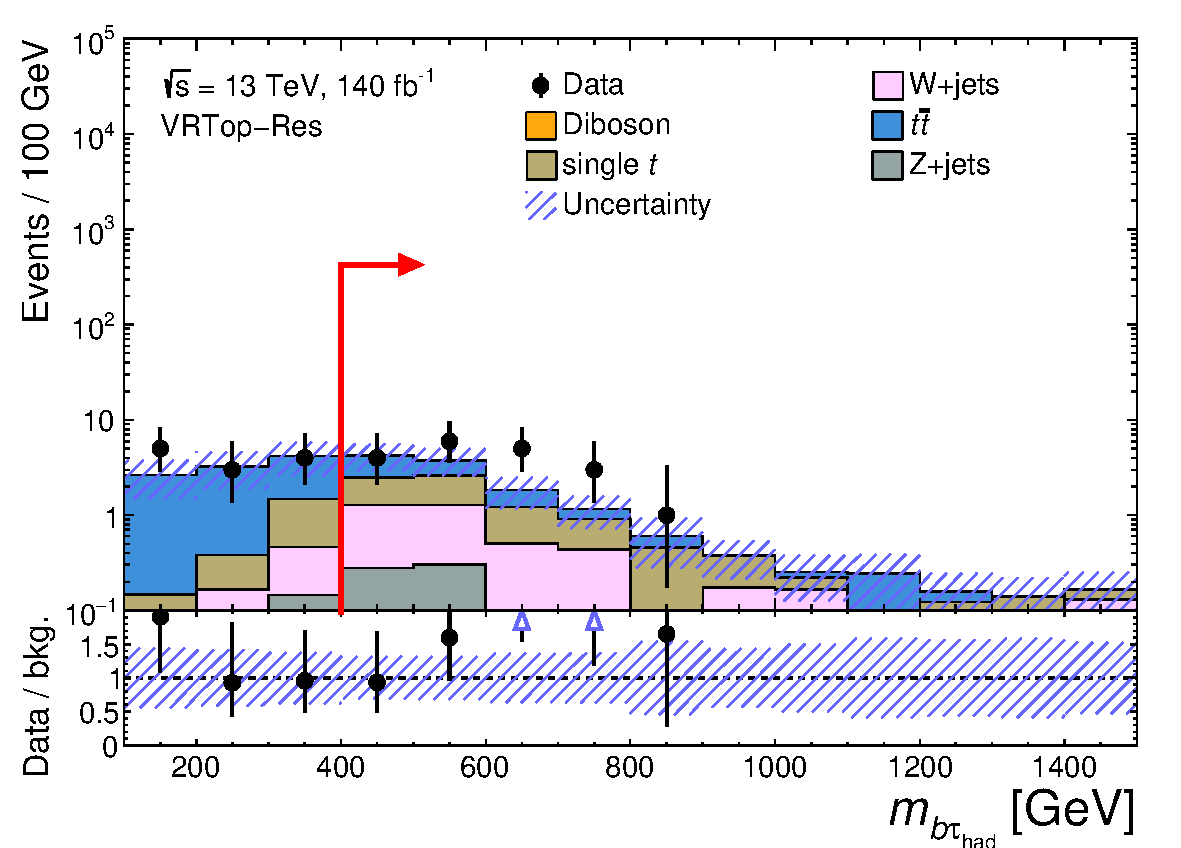
\includegraphics[width=\linewidth]{Figs/CH8/hepdata/topVR_1tau0l2b_Res_InvM_N_minus_1_Mtaub.pdf}
        \caption[]{$m_{b\hadtau}$}
    \end{subfigure}\hfill
    \begin{subfigure}{0.49\linewidth}
        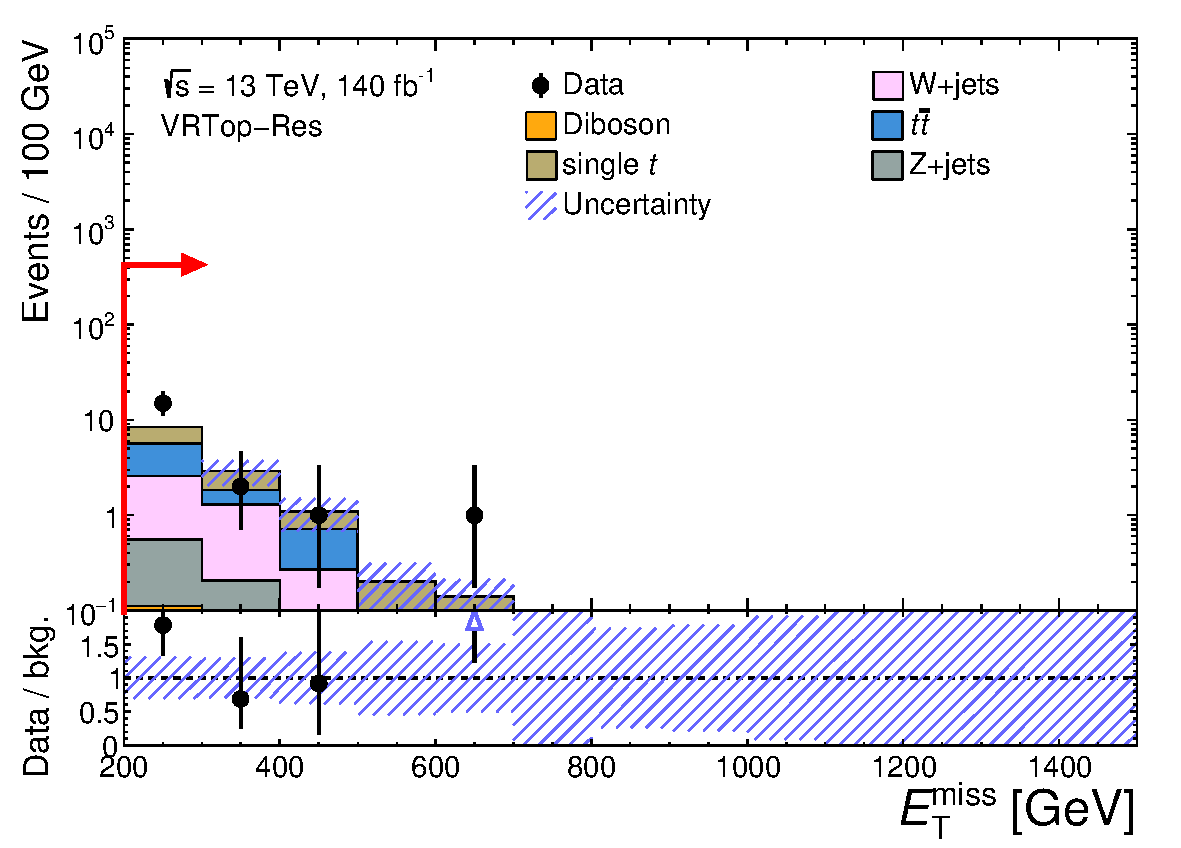
\includegraphics[width=\linewidth]{Figs/CH8/hepdata/topVR_1tau0l2b_Res_met_N_minus_1_met.pdf}
        \caption[]{$\met$}
    \end{subfigure}\\
    \begin{subfigure}{0.49\linewidth}
        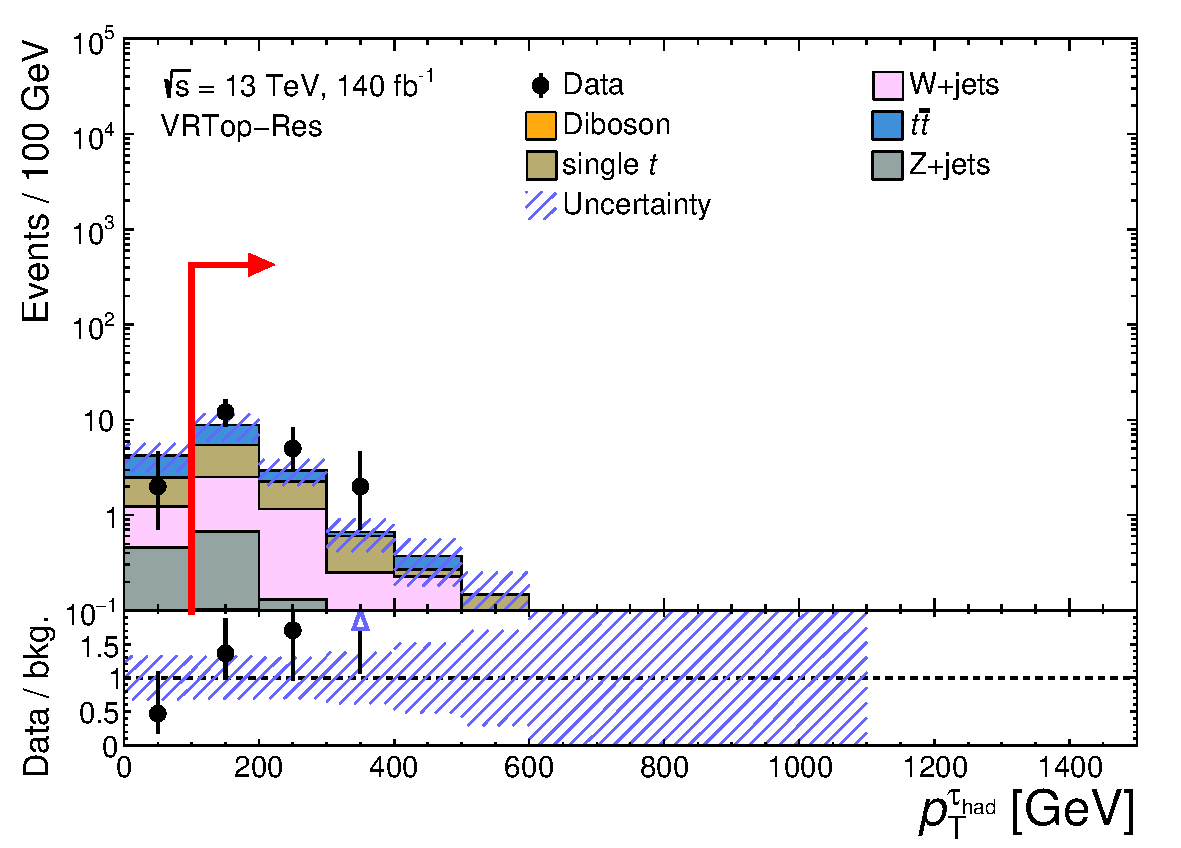
\includegraphics[width=\linewidth]{Figs/CH8/hepdata/topVR_1tau0l2b_Res_tau_pt_N_minus_1_tau_pt_0.pdf}
        \caption[]{$\pT^{\hadtau}$}
    \end{subfigure}\hfill
    \begin{subfigure}{0.49\linewidth}
        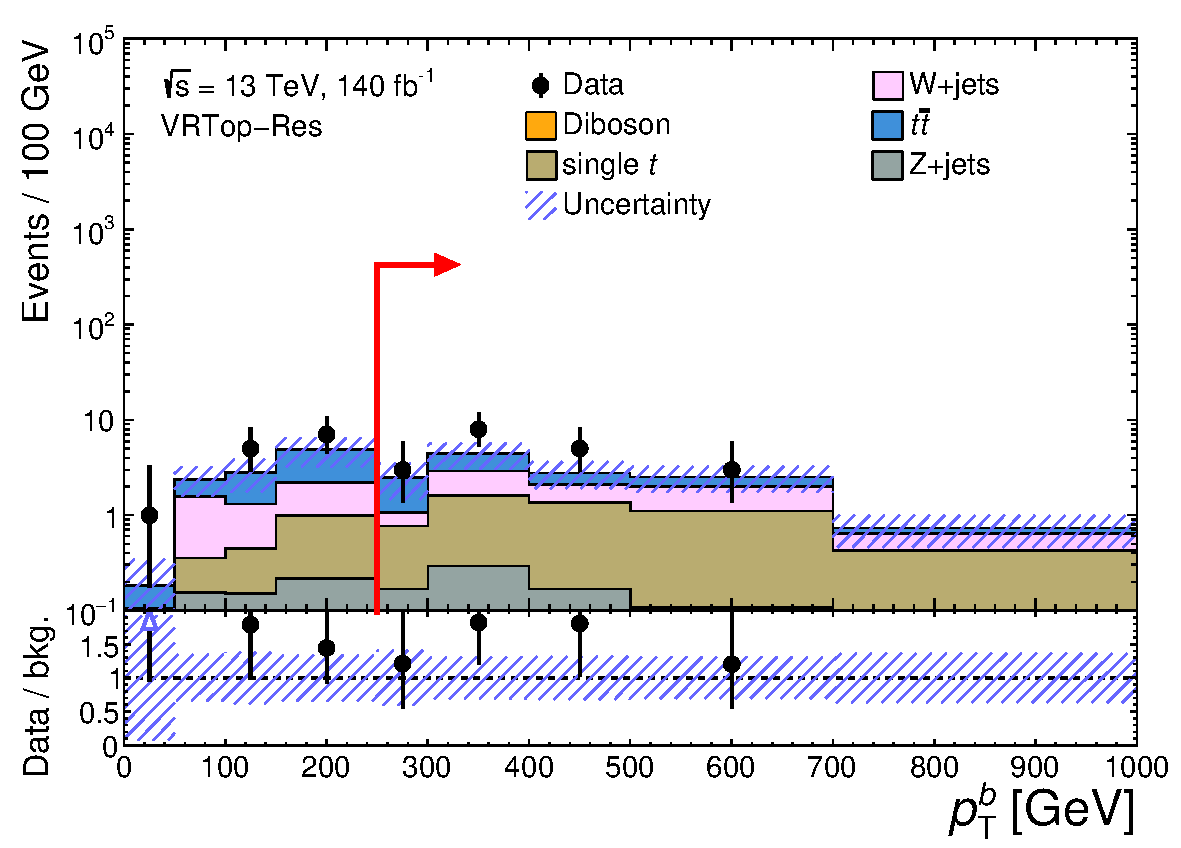
\includegraphics[width=\linewidth]{Figs/CH8/hepdata/topVR_1tau0l2b_Res_bjet_pt_N_minus_1_bjet_pt_0.pdf}
        \caption[]{$\pT^b$}
    \end{subfigure}
% Other N-1 panels retained for reference; temporarily hidden.
%     \begin{subfigure}{0.49\linewidth}
%         \includegraphics[width=\linewidth]{Figs/CH8/hepdata/topVR_1tau0l2b_Res_mT_N_minus_1_mT_tau_met.pdf}
%         \caption[]{$\mT$}
%     \end{subfigure}\\
%     \begin{subfigure}{0.49\linewidth}
%         \includegraphics[width=\linewidth]{Figs/CH8/hepdata/topVR_1tau0l2b_Res_n_bjets_N_minus_1_n_bjets.pdf}
%         \caption[]{$N_b$}
%     \end{subfigure}
    \caption[Background-only fit distributions in VRTop-Res]{$N-1$ distributions in $\VRTop$-$\Res$ after the background-only fit. The hatched bands show the combined statistical and systematic uncertainties. The bottom panels show the ratio of data to background prediction. Red arrows indicate variable thresholds for the $\VRTop$ regions. The last bin includes overflow.}
    \label{fig:ch8_vrtop_res}
\end{figure}

% Following figures are from /Users/zang/Desktop/fit_results/fit_taunub_sys_1l_allVR_BONLY_MU3000_gU2_5_23L1_0_noWeights_N_minus_1_fullRegion_v3_HEPData/Plots/
% Source files: topVR_1tau0l2b_NonRes*_postFit.eps and topVR_1tau0l2b_NonRes*_postfit.yaml.
% Local verified copies: data/ch8/hepdata_20260924/ (Plots, Histograms, Fits).
% Styling: scripts/ch8/restyle_hepdata.py --family vr; native data and ratio drawings are preserved.
% Verification: output/ch8/hepdata_vr_update_20260924/figures.json.
% Axis notation/font update: scripts/ch8/axis_labels.py; output/ch8/axis_labels_20260924/.
% Previous version: figures_vrtop_bonly_20260921.tex (selected by \CHEightCRFigureVersion).
\begin{figure}[htpb]
    \centering
    \begin{subfigure}{0.49\linewidth}
        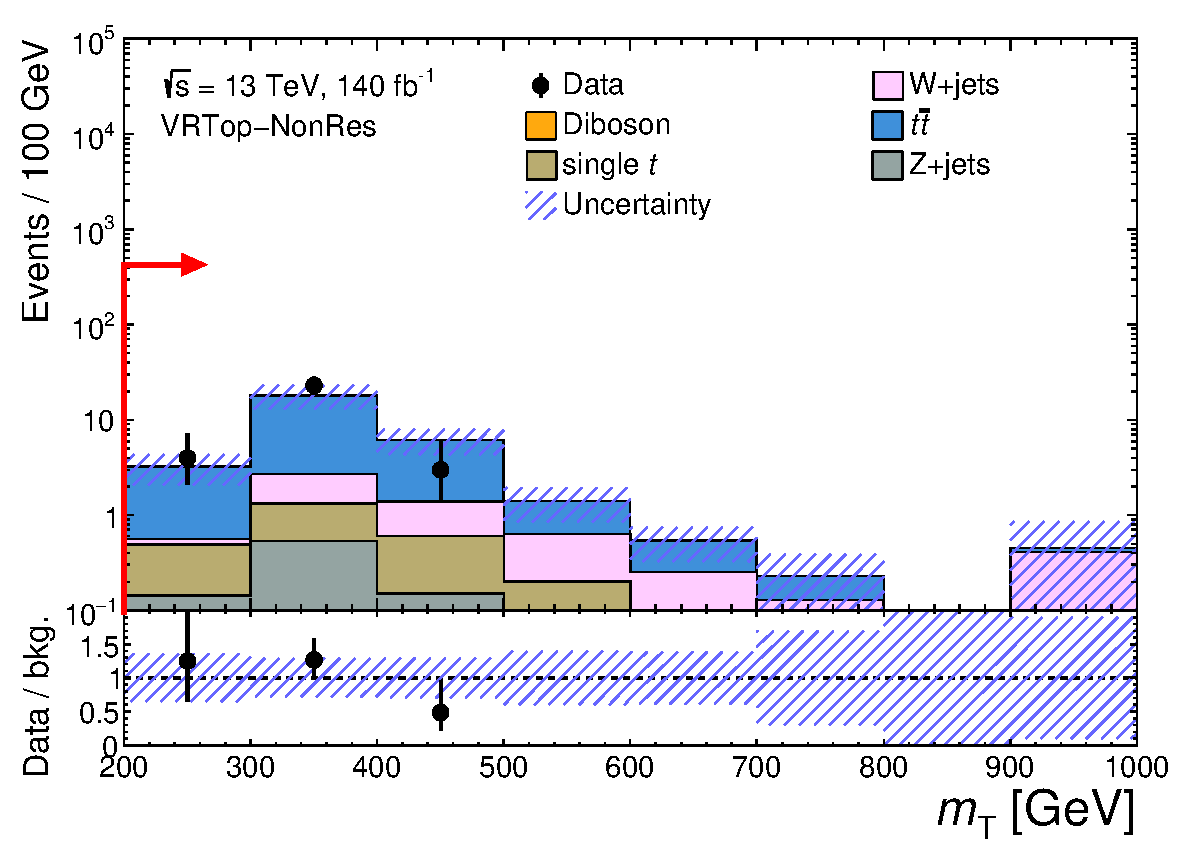
\includegraphics[width=\linewidth]{Figs/CH8/hepdata/topVR_1tau0l2b_NonRes_mT_N_minus_1_mT_tau_met.pdf}
        \caption[]{$\mT$}
    \end{subfigure}\hfill
    \begin{subfigure}{0.49\linewidth}
        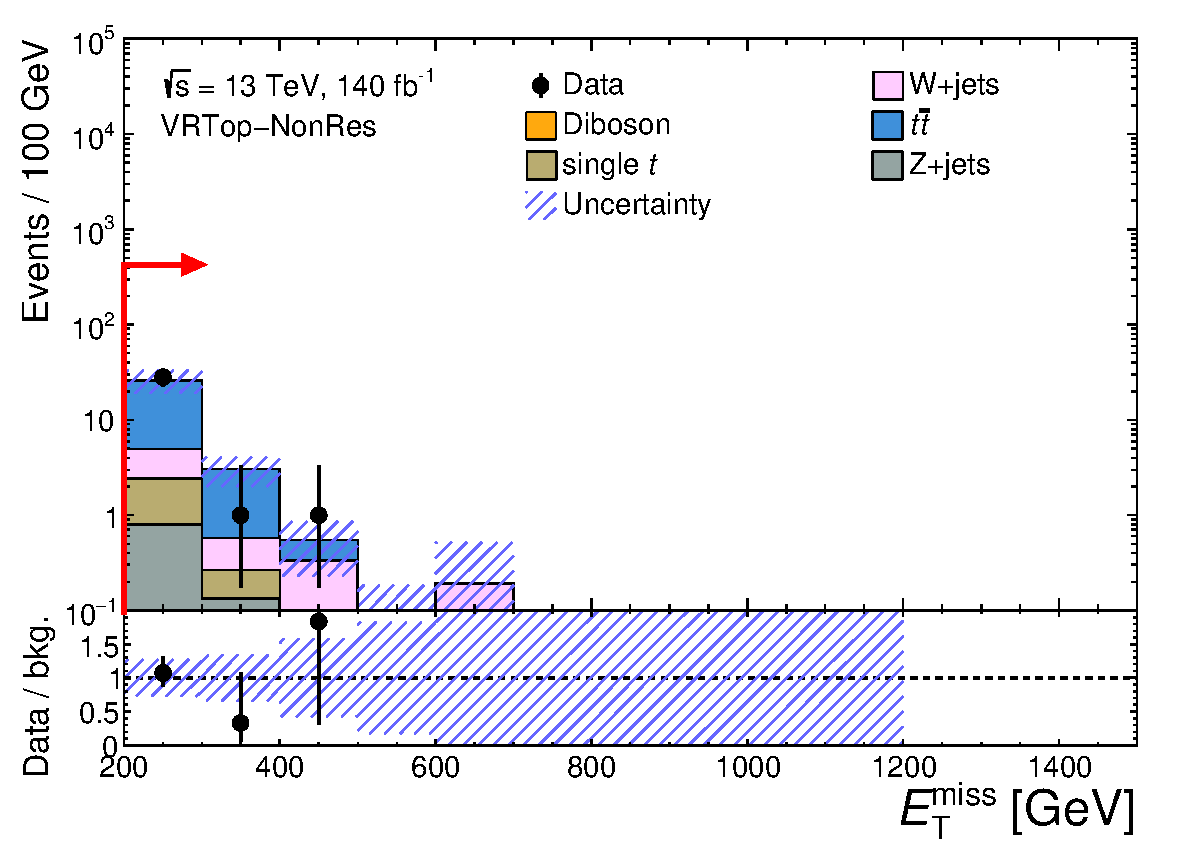
\includegraphics[width=\linewidth]{Figs/CH8/hepdata/topVR_1tau0l2b_NonRes_met_N_minus_1_met.pdf}
        \caption[]{$\met$}
    \end{subfigure}\\
    \begin{subfigure}{0.49\linewidth}
        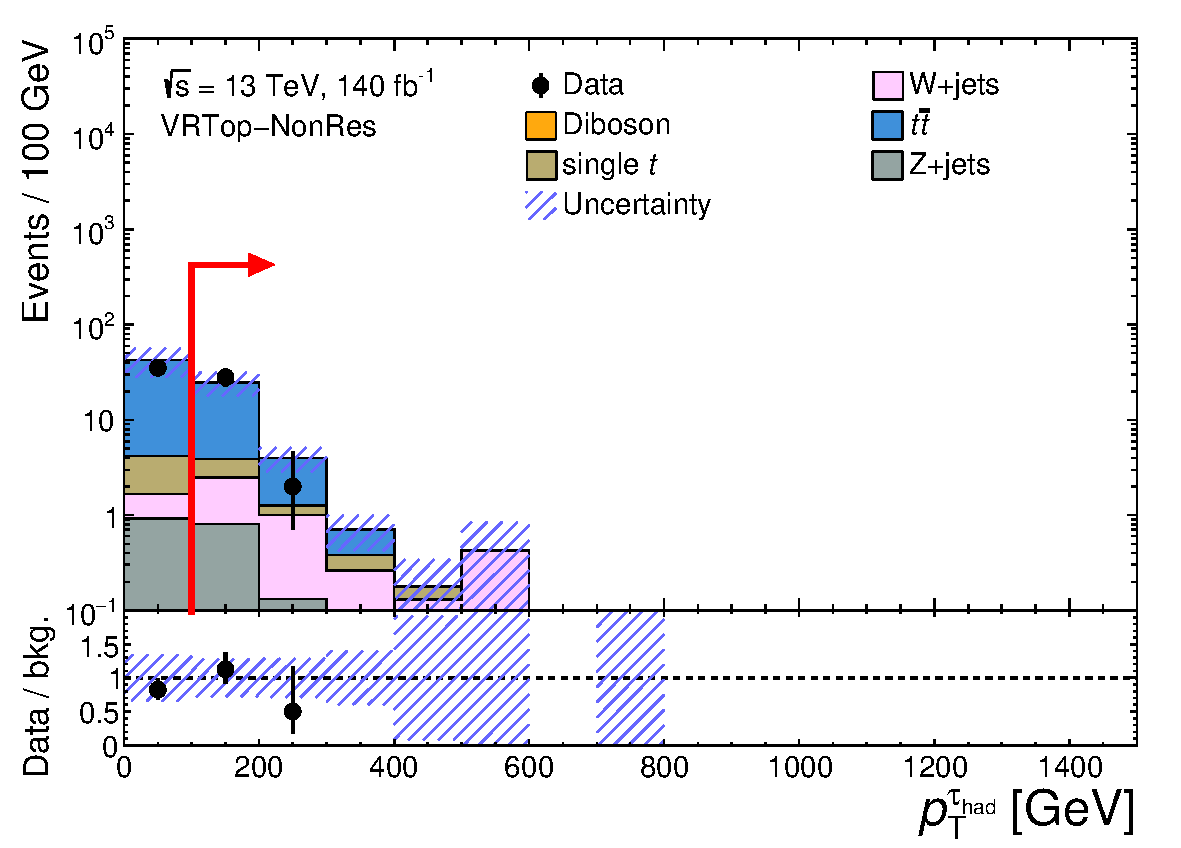
\includegraphics[width=\linewidth]{Figs/CH8/hepdata/topVR_1tau0l2b_NonRes_tau_pt_N_minus_1_tau_pt_0.pdf}
        \caption[]{$\pT^{\hadtau}$}
    \end{subfigure}\hfill
    \begin{subfigure}{0.49\linewidth}
        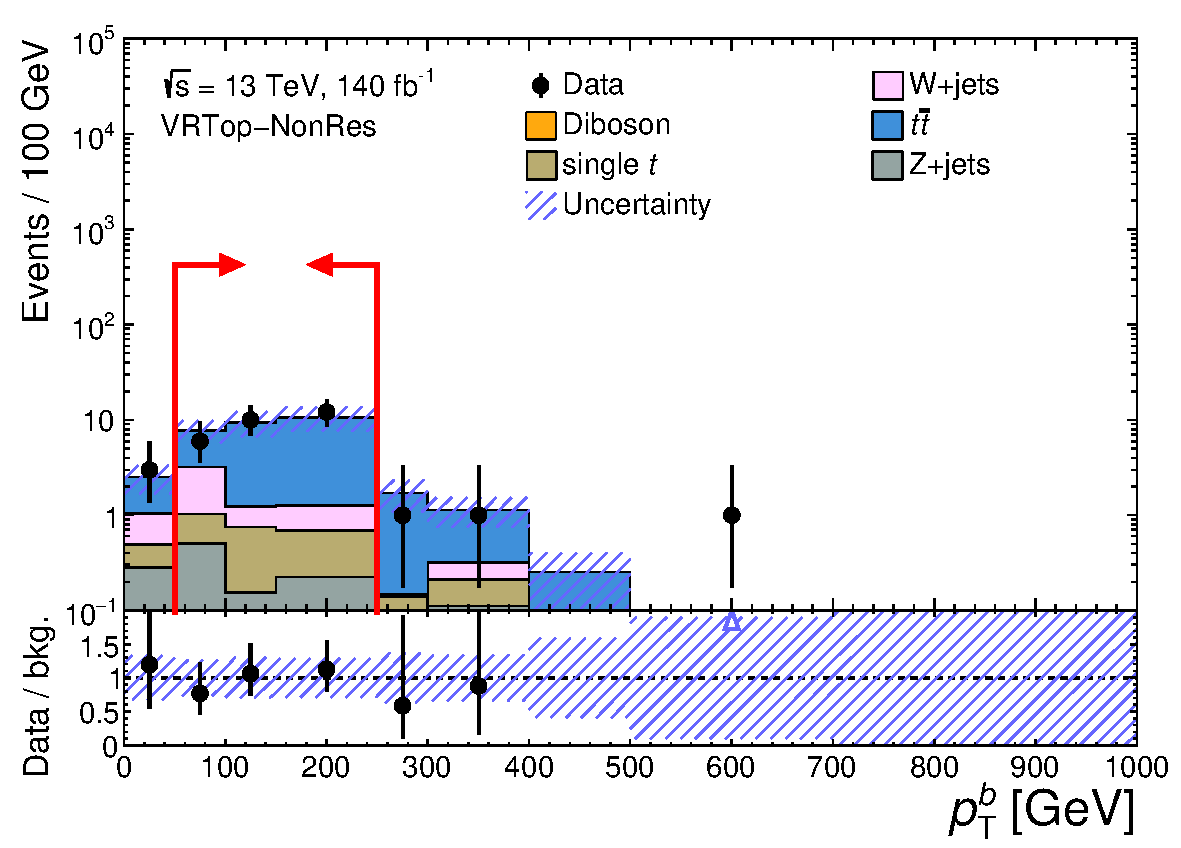
\includegraphics[width=\linewidth]{Figs/CH8/hepdata/topVR_1tau0l2b_NonRes_bjet_pt_N_minus_1_bjet_pt_0.pdf}
        \caption[]{$\pT^b$}
    \end{subfigure}
% Other N-1 panels retained for reference; temporarily hidden.
%     \begin{subfigure}{0.49\linewidth}
%         \includegraphics[width=\linewidth]{Figs/CH8/hepdata/topVR_1tau0l2b_NonRes_dphi_N_minus_1_dphi_taumet.pdf}
%         \caption[]{$\DphiTauMet$}
%     \end{subfigure}\hfill
%     \begin{subfigure}{0.49\linewidth}
%         \includegraphics[width=\linewidth]{Figs/CH8/hepdata/topVR_1tau0l2b_NonRes_n_bjets_N_minus_1_n_bjets.pdf}
%         \caption[]{$N_b$}
%     \end{subfigure}
    \caption[Background-only fit distributions in VRTop-NonRes]{$N-1$ distributions in $\VRTop$-$\NonRes$ after the background-only fit. The hatched bands show the combined statistical and systematic uncertainties. The bottom panels show the ratio of data to background prediction. Red arrows indicate variable thresholds for the $\VRTop$ regions. The last bin includes overflow.}
    \label{fig:ch8_vrtop_nonres}
\end{figure}
